\documentclass[twocolumn]{article}
\usepackage{graphicx}
\usepackage{titling}


\graphicspath{ {./imgs/} }

\title{Optimización económica de arbitraje de BESS a través de pronóstico de 
costos de mercado spot de energía en el Sistema Eléctrico Nacional chileno}
\author{Gonzalo Iglesias, Nicolás Sotelo, Max Cruz  \\
	Pontificia Universidad Católica de Chile  \\
	}

\date{\today}
% Hint: \title{what ever}, \author{who care} and \date{when ever} could stand 
% before or after the \begin{document} command 
% BUT the \maketitle command MUST come AFTER the \begin{document} command! 

\usepackage[spanish]{babel}


\begin{document}

\setlength{\droptitle}{-4em}     % Eliminate the default vertical space
\addtolength{\droptitle}{-4pt}
\maketitle


\begin{abstract}
El precio de venta de la energía (Costo Marginal o CMg) en el mercado spot chileno se determina a través del 
el costo de la unidad más cara actualmente despachada en el sub-sistema respectivo.
Para optimizar la rentabilidad de BESS que retiran e inyectan al sistema mediante el mercado
spot es crucial tener una estimación de los costos en el corto plazo (24-48 horas). Dado que el CMg depende 
principalmente de la demanda del sistema, la disponibilidad de energía renovables no convencionales y la disponibilidad
del parque convencional, sería posible realizar un pronóstico de ERNC utilizando técnicas de Machine Learning.
En este trabajo se realiza un análisis de performance de diferentes arquitecturas de redes neuronales para el pronóstico, 
incluyendo el uso de una combinación de Red Neuronal Convolucional de Grafos (GCN) y
RNN/GRU/LSTM; un Transformer para series temporales; y un modelo híbrido Transformer + CNN para
capturar patrones estacionales y relaciones de largo alcance.
 \ldots
\end{abstract}

\section{Introducción}
Durante la última decada, Chile ha experimentado un rápido crecimiento en la penetración de
 energías renovables no convencionales (ERNC), en particular en la zona norte, como se observa en la figura \ref{fig:matriz_sistema}
 , el cual no ha sido acompañado en la misma medida por un aumento
 en la capacidad de transmisión, cuyos proyectos tienen un tiempo de desarrollo significativamente mayor.
 Esto ha llevado a que el sistema eléctrico nacional (SEN) se vea afectado por congestiones de transmisión, las cuales no dan 
 abasto para llevar toda la energía producida en la zona norte del país a las zonas centrales donde hay mayores consumos.
 Esta condición de exceso de oferta de energía en la zona norte conlleva el CMg de la zona afectada se desplome y que las 
 centrales ERNC deban disminuir su producción de energia en un fenonemo conocido como \textit{vertimiento} o \textit{curtailment}.
 
\begin{figure}[htbp]
    \centering
    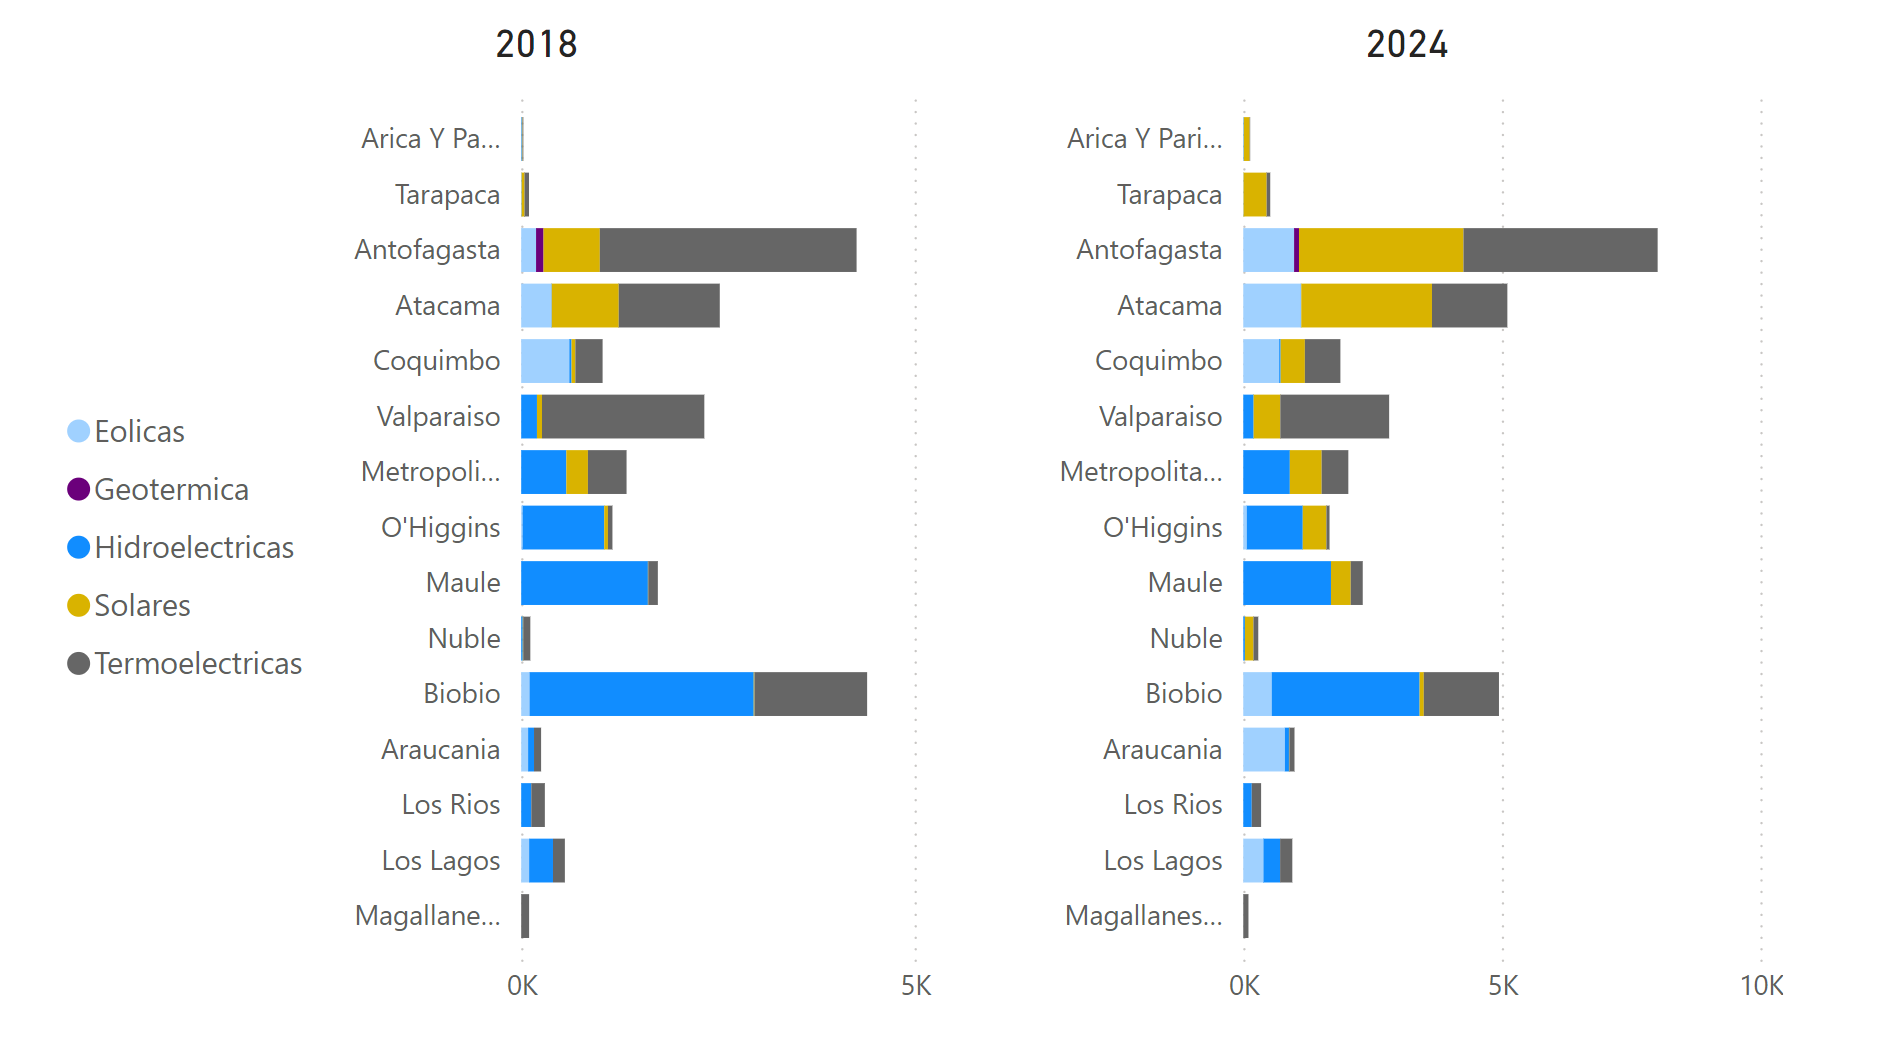
\includegraphics[width=1\columnwidth]{matriz_sist.png}
    \caption{Cambio en la Matriz de Generación del SEN}
    \label{fig:matriz_sistema}
\end{figure}

\paragraph{}
La disminución de la producción y la baja de los CMg afectan por partida doble la rentabilidad de las centrales ERNC, ya que
no solo inyectan menos energía, sino que la que logran entregar al sistema se vende a costo muy bajo o 0.
Estas escenario ha generado otro boom en la industria, que busca aminorar estos efectos a traves del desarrollo de 
proyectos de almacenamiento de energía (BESS) que les permitirá almacenar la energía generada en horas de exceso de esta 
e inyectarla en horas donde hay mejores precios. Pero para rentabilizar estos proyectos es necesario maximizar el spread
del CMg, es decir, comprar la energía en las horas de menor precio y luego venderla en las de mayor CMg. Para esto,
trabajaremos con distintos modelos, de modo de identificar la arquitectura que mejor se adapte a la tarea del pronóstico 
de los costos.

\begin{figure}[htbp]
    \centering
    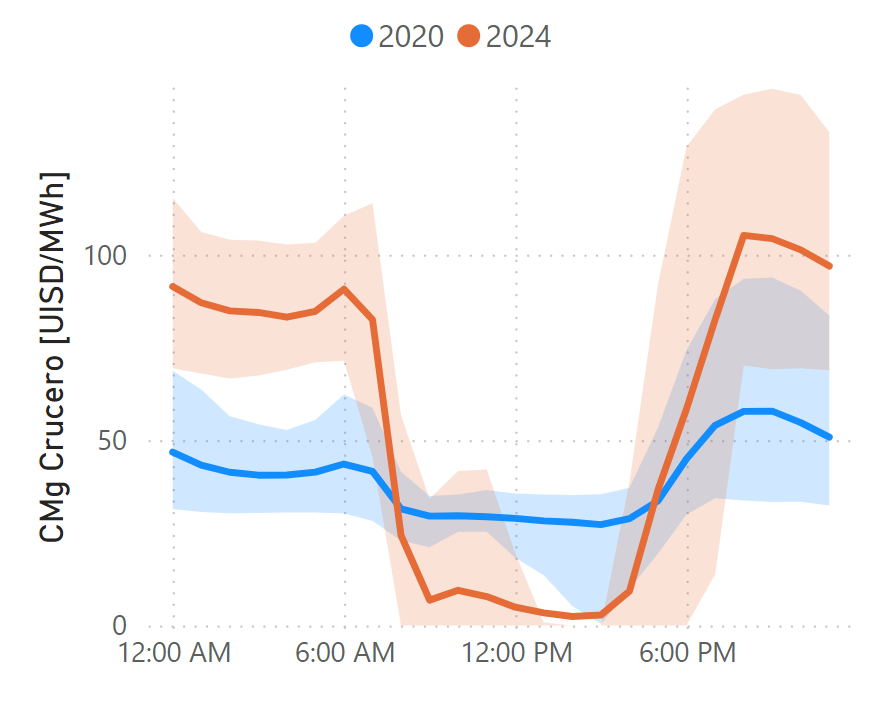
\includegraphics[width=0.8\columnwidth]{cmg_comparacion.png}
    \caption{Comparación perfil diario CMg promedio pre y post escenario de congestión em barra
	Crucero 220kV}
    \label{fig:comp_cmg}
\end{figure}


\section{Metodología}

\subsection{Datos}
Para la el entrenamiento de los modelos, contamos con una serie de datos
los cuales son considerados drivers claves del costo marginal, adicionales al CMg histórico
el cual será nuestra variable objetivo.

\begin{itemize}
    \item Demanda Nacional
    
    Valores historicos de la demanda electrica nacional en MW desde el 2018 a la fecha y con
	resolución horaria.

    \item Disponibilida ERNC
    
    Pronóstico histórico de la disponibilidad de ERNC en MW por central 
	desde el 2018 a la fecha y con
	resolución horaria.

    \item Matriz de Generación
    
	Potencia instalada por tecnología en MW a lo largo del tiempo desde 2018 hasta la fecha.

    \item Cotas de Embalse
    
	Cotas de embalse de las principales centrales hidroeléctricas del sistema.
\end{itemize}

La combinación de estos datos, con distintas escalas de estaicionalidad, nos entregarán unas condiciones
de borde importantes para el pronóstico del CMg.

\subsection{Modelos}
Para abordar el problema, se compararan tres arquitecturas de deep learning, en las que se busca
un enfoque novedoso para enfrentar este problema de series de tiempo:

\begin{enumerate}
    \item Red Neuronal Convolucional de Grafos
	(GCN) + RNN/GRU/LSTM

	Esta arquitectura combina una GCN para modelar la red de
	transmision electrica y capturar interacciones espaciales, 
	con una capa recurrente (RNN o GRU) para
	modelar las dependencias temporales. Los nodos
	en la GCN representan subestaciones, y las aristas representan las líneas de
	transmision y sus restricciones de capacidad.

    \item Transformer para Series Temporales
    
	Transformers se aplicaran a los datos de series temporales para 
	capturar patrones de largo plazo y
	relaciones temporales en el CMg y la demanda energetica. 
	La atencion temporal permitira que el
	modelo identifique eventos críticos en la serie de precios y prediga
	 tendencias a largo plazo.

    \item Transformers + CNN para Series Temporales

	Este enfoque combinara la capacidad de las
	CNNs para extraer patrones locales en series temporales 
	(como estacionalidades intradía) con la capacidad de los 
	Transformers para capturar relaciones
	temporales de largo alcance, permitiendo una 
	representacion robusta de los datos temporales y la variabilidad de los precios.
    
\end{enumerate}




% \section{Conclusions}\label{conclusions}
% There is no longer \LaTeX{} example which was written by \cite{doe}.


% \begin{thebibliography}{9}
% \bibitem[Doe]{doe} \emph{First and last \LaTeX{} example.},
% John Doe 50 B.C. 
% \end{thebibliography}

\end{document}